\documentclass[1p]{elsarticle_modified}
%\bibliographystyle{elsarticle-num}

%\usepackage[colorlinks]{hyperref}
%\usepackage{abbrmath_seonhwa} %\Abb, \Ascr, \Acal ,\Abf, \Afrak
\usepackage{amsfonts}
\usepackage{amssymb}
\usepackage{amsmath}
\usepackage{amsthm}
\usepackage{scalefnt}
\usepackage{amsbsy}
\usepackage{kotex}
\usepackage{caption}
\usepackage{subfig}
\usepackage{color}
\usepackage{graphicx}
\usepackage{xcolor} %% white, black, red, green, blue, cyan, magenta, yellow
\usepackage{float}
\usepackage{setspace}
\usepackage{hyperref}

\usepackage{tikz}
\usetikzlibrary{arrows}

\usepackage{multirow}
\usepackage{array} % fixed length table
\usepackage{hhline}

%%%%%%%%%%%%%%%%%%%%%
\makeatletter
\renewcommand*\env@matrix[1][\arraystretch]{%
	\edef\arraystretch{#1}%
	\hskip -\arraycolsep
	\let\@ifnextchar\new@ifnextchar
	\array{*\c@MaxMatrixCols c}}
\makeatother %https://tex.stackexchange.com/questions/14071/how-can-i-increase-the-line-spacing-in-a-matrix
%%%%%%%%%%%%%%%

\usepackage[normalem]{ulem}

\newcommand{\msout}[1]{\ifmmode\text{\sout{\ensuremath{#1}}}\else\sout{#1}\fi}
%SOURCE: \msout is \stkout macro in https://tex.stackexchange.com/questions/20609/strikeout-in-math-mode

\newcommand{\cancel}[1]{
	\ifmmode
	{\color{red}\msout{#1}}
	\else
	{\color{red}\sout{#1}}
	\fi
}

\newcommand{\add}[1]{
	{\color{blue}\uwave{#1}}
}

\newcommand{\replace}[2]{
	\ifmmode
	{\color{red}\msout{#1}}{\color{blue}\uwave{#2}}
	\else
	{\color{red}\sout{#1}}{\color{blue}\uwave{#2}}
	\fi
}

\newcommand{\Sol}{\mathcal{S}} %segment
\newcommand{\D}{D} %diagram
\newcommand{\A}{\mathcal{A}} %arc


%%%%%%%%%%%%%%%%%%%%%%%%%%%%%5 test

\def\sl{\operatorname{\textup{SL}}(2,\Cbb)}
\def\psl{\operatorname{\textup{PSL}}(2,\Cbb)}
\def\quan{\mkern 1mu \triangleright \mkern 1mu}

\theoremstyle{definition}
\newtheorem{thm}{Theorem}[section]
\newtheorem{prop}[thm]{Proposition}
\newtheorem{lem}[thm]{Lemma}
\newtheorem{ques}[thm]{Question}
\newtheorem{cor}[thm]{Corollary}
\newtheorem{defn}[thm]{Definition}
\newtheorem{exam}[thm]{Example}
\newtheorem{rmk}[thm]{Remark}
\newtheorem{alg}[thm]{Algorithm}

\newcommand{\I}{\sqrt{-1}}
\begin{document}

%\begin{frontmatter}
%
%\title{Boundary parabolic representations of knots up to 8 crossings}
%
%%% Group authors per affiliation:
%\author{Yunhi Cho} 
%\address{Department of Mathematics, University of Seoul, Seoul, Korea}
%\ead{yhcho@uos.ac.kr}
%
%
%\author{Seonhwa Kim} %\fnref{s_kim}}
%\address{Center for Geometry and Physics, Institute for Basic Science, Pohang, 37673, Korea}
%\ead{ryeona17@ibs.re.kr}
%
%\author{Hyuk Kim}
%\address{Department of Mathematical Sciences, Seoul National University, Seoul 08826, Korea}
%\ead{hyukkim@snu.ac.kr}
%
%\author{Seokbeom Yoon}
%\address{Department of Mathematical Sciences, Seoul National University, Seoul, 08826,  Korea}
%\ead{sbyoon15@snu.ac.kr}
%
%\begin{abstract}
%We find all boundary parabolic representation of knots up to 8 crossings.
%
%\end{abstract}
%\begin{keyword}
%    \MSC[2010] 57M25 
%\end{keyword}
%
%\end{frontmatter}

%\linenumbers
%\tableofcontents
%
\newcommand\colored[1]{\textcolor{white}{\rule[-0.35ex]{0.8em}{1.4ex}}\kern-0.8em\color{red} #1}%
%\newcommand\colored[1]{\textcolor{white}{ #1}\kern-2.17ex	\textcolor{white}{ #1}\kern-1.81ex	\textcolor{white}{ #1}\kern-2.15ex\color{red}#1	}

{\Large $\underline{12a_{0764}~(K12a_{0764})}$}

\setlength{\tabcolsep}{10pt}
\renewcommand{\arraystretch}{1.6}
\vspace{1cm}\begin{tabular}{m{100pt}>{\centering\arraybackslash}m{274pt}}
\multirow{5}{120pt}{
	\centering
	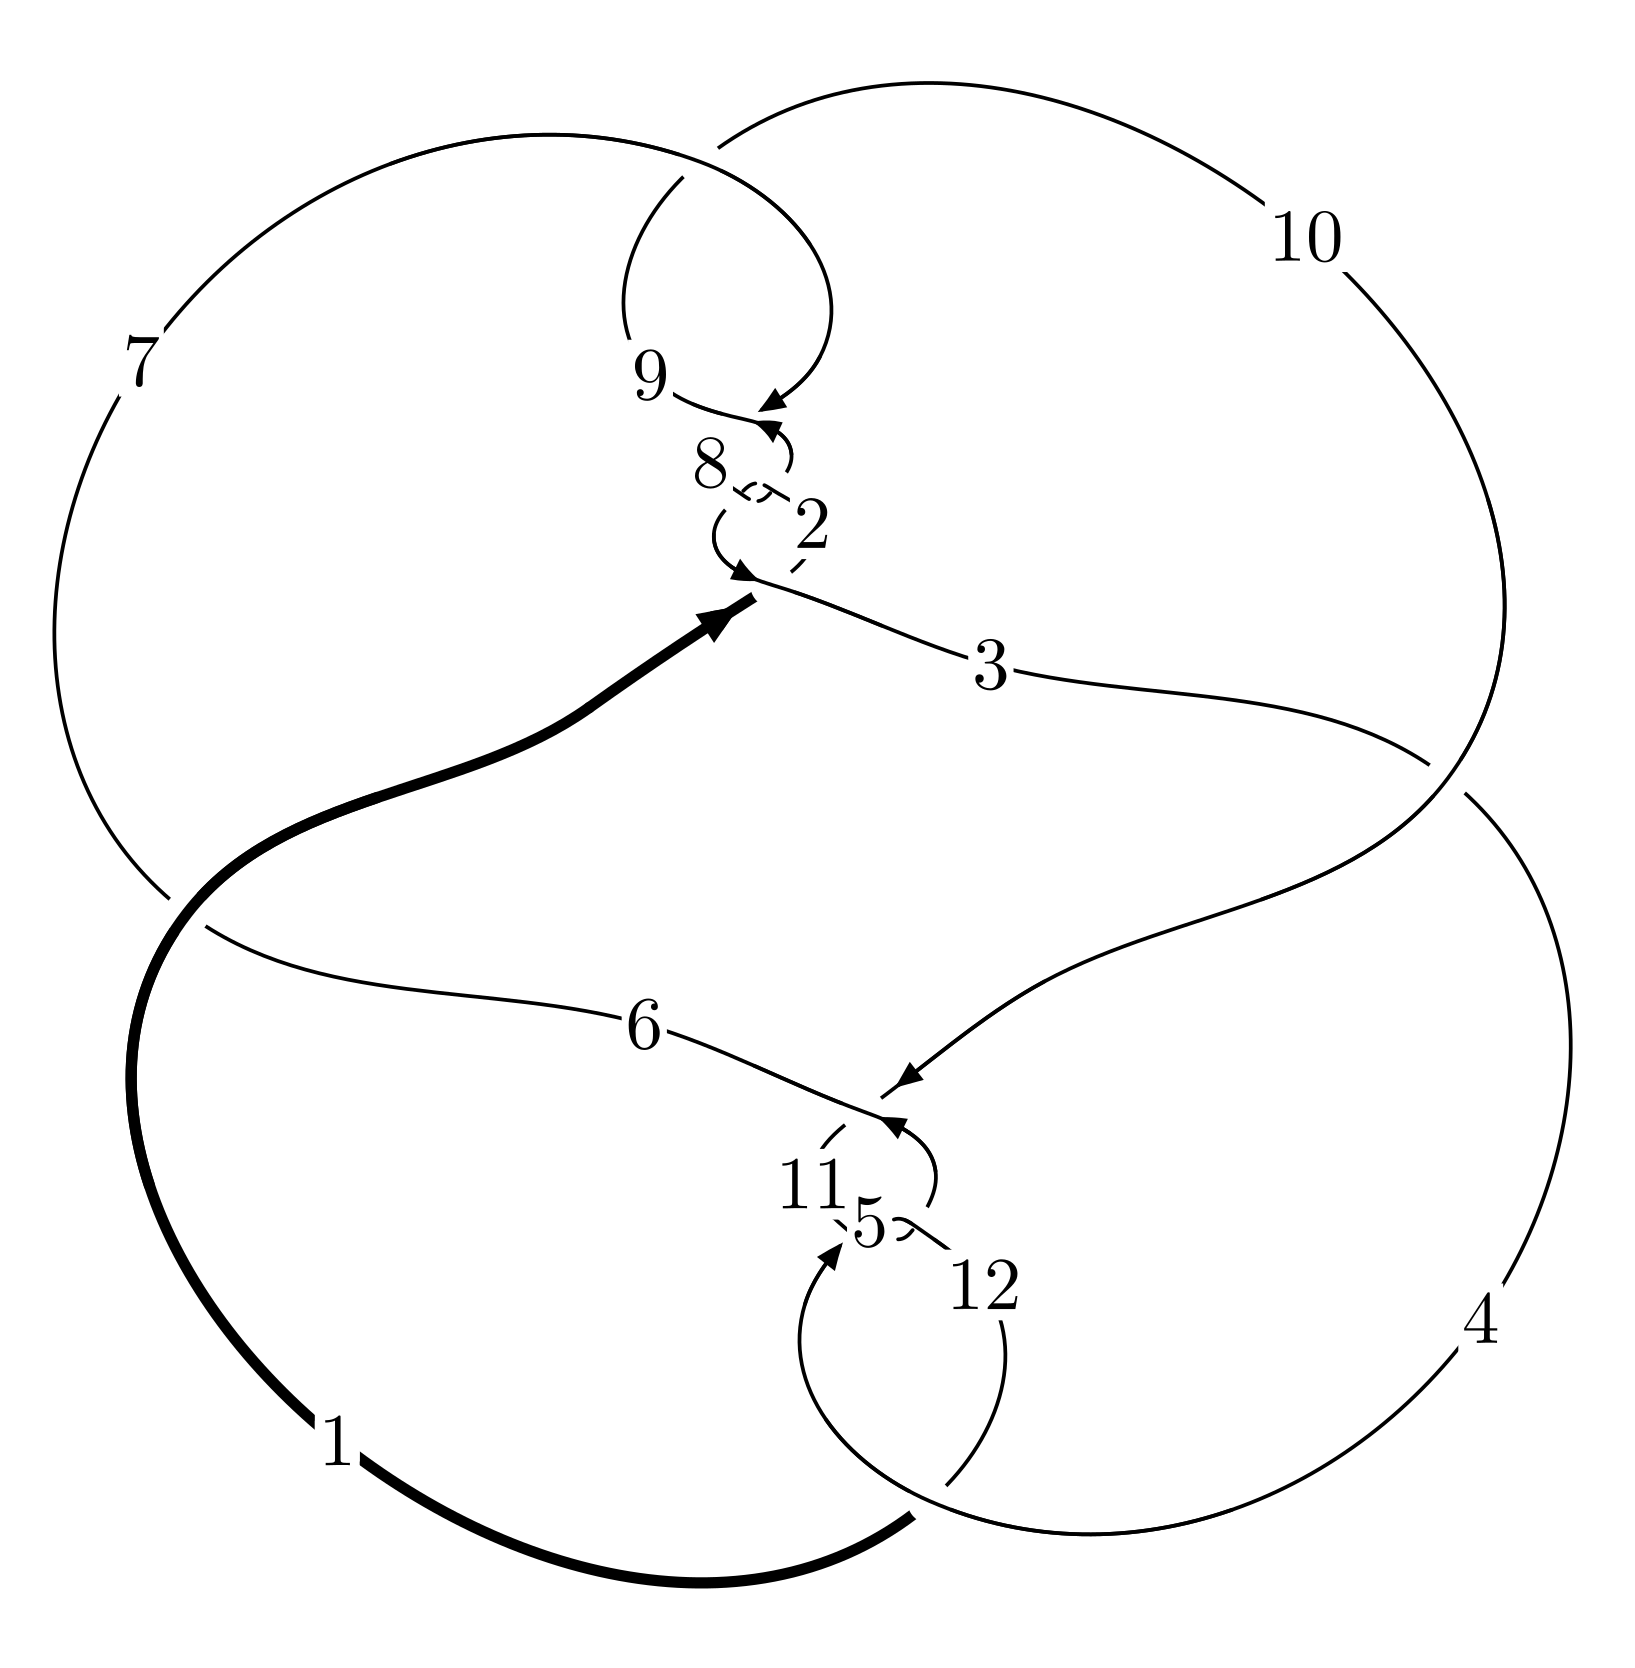
\includegraphics[width=112pt]{../../../GIT/diagram.site/Diagrams/png/1565_12a_0764.png}\\
\ \ \ A knot diagram\footnotemark}&
\allowdisplaybreaks
\textbf{Linearized knot diagam} \\
\cline{2-2}
 &
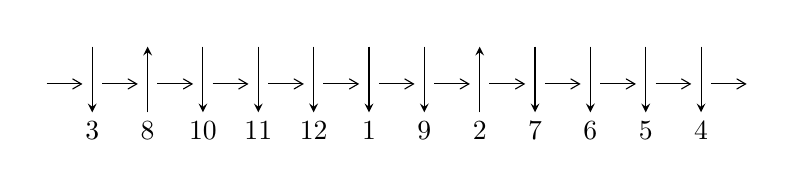
\begin{tikzpicture}[x=20pt, y=17pt]
	% nodes
	\node (C0) at (0, 0) {};
	\node (C1) at (1, 0) {};
	\node (C1U) at (1, +1) {};
	\node (C1D) at (1, -1) {3};

	\node (C2) at (2, 0) {};
	\node (C2U) at (2, +1) {};
	\node (C2D) at (2, -1) {8};

	\node (C3) at (3, 0) {};
	\node (C3U) at (3, +1) {};
	\node (C3D) at (3, -1) {10};

	\node (C4) at (4, 0) {};
	\node (C4U) at (4, +1) {};
	\node (C4D) at (4, -1) {11};

	\node (C5) at (5, 0) {};
	\node (C5U) at (5, +1) {};
	\node (C5D) at (5, -1) {12};

	\node (C6) at (6, 0) {};
	\node (C6U) at (6, +1) {};
	\node (C6D) at (6, -1) {1};

	\node (C7) at (7, 0) {};
	\node (C7U) at (7, +1) {};
	\node (C7D) at (7, -1) {9};

	\node (C8) at (8, 0) {};
	\node (C8U) at (8, +1) {};
	\node (C8D) at (8, -1) {2};

	\node (C9) at (9, 0) {};
	\node (C9U) at (9, +1) {};
	\node (C9D) at (9, -1) {7};

	\node (C10) at (10, 0) {};
	\node (C10U) at (10, +1) {};
	\node (C10D) at (10, -1) {6};

	\node (C11) at (11, 0) {};
	\node (C11U) at (11, +1) {};
	\node (C11D) at (11, -1) {5};

	\node (C12) at (12, 0) {};
	\node (C12U) at (12, +1) {};
	\node (C12D) at (12, -1) {4};
	\node (C13) at (13, 0) {};

	% arrows
	\draw[->,>={angle 60}]
	(C0) edge (C1) (C1) edge (C2) (C2) edge (C3) (C3) edge (C4) (C4) edge (C5) (C5) edge (C6) (C6) edge (C7) (C7) edge (C8) (C8) edge (C9) (C9) edge (C10) (C10) edge (C11) (C11) edge (C12) (C12) edge (C13) ;	\draw[->,>=stealth]
	(C1U) edge (C1D) (C2D) edge (C2U) (C3U) edge (C3D) (C4U) edge (C4D) (C5U) edge (C5D) (C6U) edge (C6D) (C7U) edge (C7D) (C8D) edge (C8U) (C9U) edge (C9D) (C10U) edge (C10D) (C11U) edge (C11D) (C12U) edge (C12D) ;
	\end{tikzpicture} \\
\hhline{~~} \\& 
\textbf{Solving Sequence} \\ \cline{2-2} 
 &
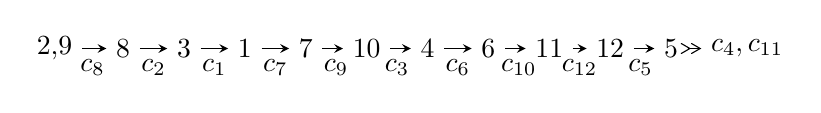
\begin{tikzpicture}[x=22pt, y=7pt]
	% node
	\node (A0) at (-1/8, 0) {2,9};
	\node (A1) at (1, 0) {8};
	\node (A2) at (2, 0) {3};
	\node (A3) at (3, 0) {1};
	\node (A4) at (4, 0) {7};
	\node (A5) at (5, 0) {10};
	\node (A6) at (6, 0) {4};
	\node (A7) at (7, 0) {6};
	\node (A8) at (8, 0) {11};
	\node (A9) at (9, 0) {12};
	\node (A10) at (10, 0) {5};
	\node (C1) at (1/2, -1) {$c_{8}$};
	\node (C2) at (3/2, -1) {$c_{2}$};
	\node (C3) at (5/2, -1) {$c_{1}$};
	\node (C4) at (7/2, -1) {$c_{7}$};
	\node (C5) at (9/2, -1) {$c_{9}$};
	\node (C6) at (11/2, -1) {$c_{3}$};
	\node (C7) at (13/2, -1) {$c_{6}$};
	\node (C8) at (15/2, -1) {$c_{10}$};
	\node (C9) at (17/2, -1) {$c_{12}$};
	\node (C10) at (19/2, -1) {$c_{5}$};
	\node (A11) at (45/4, 0) {$c_{4},c_{11}$};

	% edge
	\draw[->,>=stealth]	
	(A0) edge (A1) (A1) edge (A2) (A2) edge (A3) (A3) edge (A4) (A4) edge (A5) (A5) edge (A6) (A6) edge (A7) (A7) edge (A8) (A8) edge (A9) (A9) edge (A10) ;
	\draw[->>,>={angle 60}]	
	(A10) edge (A11);
\end{tikzpicture} \\ 

\end{tabular} \\

\footnotetext{
The image of knot diagram is generated by the software ``\textbf{Draw programme}" developed by Andrew Bartholomew(\url{http://www.layer8.co.uk/maths/draw/index.htm\#Running-draw}), where we modified some parts for our purpose(\url{https://github.com/CATsTAILs/LinksPainter}).
}\phantom \\ \newline 
\centering \textbf{Ideals for irreducible components\footnotemark of $X_{\text{par}}$} 
 
\begin{align*}
I^u_{1}&=\langle 
u^{66}- u^{65}+\cdots- u-1\rangle \\
\\
\end{align*}
\raggedright * 1 irreducible components of $\dim_{\mathbb{C}}=0$, with total 66 representations.\\
\footnotetext{All coefficients of polynomials are rational numbers. But the coefficients are sometimes approximated in decimal forms when there is not enough margin.}
\newpage
\renewcommand{\arraystretch}{1}
\centering \section*{I. $I^u_{1}= \langle u^{66}- u^{65}+\cdots- u-1 \rangle$}
\flushleft \textbf{(i) Arc colorings}\\
\begin{tabular}{m{7pt} m{180pt} m{7pt} m{180pt} }
\flushright $a_{2}=$&$\begin{pmatrix}0\\u\end{pmatrix}$ \\
\flushright $a_{9}=$&$\begin{pmatrix}1\\0\end{pmatrix}$ \\
\flushright $a_{8}=$&$\begin{pmatrix}1\\u^2\end{pmatrix}$ \\
\flushright $a_{3}=$&$\begin{pmatrix}u\\u^3+u\end{pmatrix}$ \\
\flushright $a_{1}=$&$\begin{pmatrix}u^3\\u^5+u^3+u\end{pmatrix}$ \\
\flushright $a_{7}=$&$\begin{pmatrix}u^2+1\\u^2\end{pmatrix}$ \\
\flushright $a_{10}=$&$\begin{pmatrix}u^4+u^2+1\\u^4\end{pmatrix}$ \\
\flushright $a_{4}=$&$\begin{pmatrix}- u^{11}-2 u^9-4 u^7-4 u^5-3 u^3\\- u^{11}- u^9-2 u^7- u^5+u^3+u\end{pmatrix}$ \\
\flushright $a_{6}=$&$\begin{pmatrix}- u^{10}- u^8-2 u^6- u^4+u^2+1\\- u^{12}-2 u^{10}-4 u^8-4 u^6-3 u^4\end{pmatrix}$ \\
\flushright $a_{11}=$&$\begin{pmatrix}u^{26}+3 u^{24}+\cdots+u^2+1\\u^{28}+4 u^{26}+\cdots+12 u^8+u^4\end{pmatrix}$ \\
\flushright $a_{12}=$&$\begin{pmatrix}u^{27}+4 u^{25}+\cdots+12 u^7+u^3\\u^{27}+3 u^{25}+\cdots+u^3+u\end{pmatrix}$ \\
\flushright $a_{5}=$&$\begin{pmatrix}- u^{65}-8 u^{63}+\cdots-6 u^3- u\\- u^{65}+u^{64}+\cdots- u-1\end{pmatrix}$\\&\end{tabular}
\flushleft \textbf{(ii) Obstruction class $= -1$}\\~\\
\flushleft \textbf{(iii) Cusp Shapes $= 4 u^{65}+32 u^{63}+\cdots-16 u-14$}\\~\\
\newpage\renewcommand{\arraystretch}{1}
\flushleft \textbf{(iv) u-Polynomials at the component}\newline \\
\begin{tabular}{m{50pt}|m{274pt}}
Crossings & \hspace{64pt}u-Polynomials at each crossing \\
\hline $$\begin{aligned}c_{1},c_{7},c_{9}\end{aligned}$$&$\begin{aligned}
&u^{66}+17 u^{65}+\cdots+u+1
\end{aligned}$\\
\hline $$\begin{aligned}c_{2},c_{8}\end{aligned}$$&$\begin{aligned}
&u^{66}- u^{65}+\cdots- u-1
\end{aligned}$\\
\hline $$\begin{aligned}c_{3},c_{6}\end{aligned}$$&$\begin{aligned}
&u^{66}- u^{65}+\cdots-36 u-40
\end{aligned}$\\
\hline $$\begin{aligned}c_{4},c_{5},c_{11}\end{aligned}$$&$\begin{aligned}
&u^{66}+u^{65}+\cdots-3 u-1
\end{aligned}$\\
\hline $$\begin{aligned}c_{10},c_{12}\end{aligned}$$&$\begin{aligned}
&u^{66}-3 u^{65}+\cdots+3 u+3
\end{aligned}$\\
\hline
\end{tabular}\\~\\
\newpage\renewcommand{\arraystretch}{1}
\flushleft \textbf{(v) Riley Polynomials at the component}\newline \\
\begin{tabular}{m{50pt}|m{274pt}}
Crossings & \hspace{64pt}Riley Polynomials at each crossing \\
\hline $$\begin{aligned}c_{1},c_{7},c_{9}\end{aligned}$$&$\begin{aligned}
&y^{66}+65 y^{65}+\cdots-31 y+1
\end{aligned}$\\
\hline $$\begin{aligned}c_{2},c_{8}\end{aligned}$$&$\begin{aligned}
&y^{66}+17 y^{65}+\cdots+y+1
\end{aligned}$\\
\hline $$\begin{aligned}c_{3},c_{6}\end{aligned}$$&$\begin{aligned}
&y^{66}-35 y^{65}+\cdots-32496 y+1600
\end{aligned}$\\
\hline $$\begin{aligned}c_{4},c_{5},c_{11}\end{aligned}$$&$\begin{aligned}
&y^{66}-55 y^{65}+\cdots+y+1
\end{aligned}$\\
\hline $$\begin{aligned}c_{10},c_{12}\end{aligned}$$&$\begin{aligned}
&y^{66}+37 y^{65}+\cdots-3 y+9
\end{aligned}$\\
\hline
\end{tabular}\\~\\
\newpage\flushleft \textbf{(vi) Complex Volumes and Cusp Shapes}
$$\begin{array}{c|c|c}  
\text{Solutions to }I^u_{1}& \I (\text{vol} + \sqrt{-1}CS) & \text{Cusp shape}\\
 \hline 
\begin{aligned}
u &= -0.207533 + 0.981086 I\end{aligned}
 & -6.35096 + 4.33929 I & -15.3912 - 1.6731 I \\ \hline\begin{aligned}
u &= -0.207533 - 0.981086 I\end{aligned}
 & -6.35096 - 4.33929 I & -15.3912 + 1.6731 I \\ \hline\begin{aligned}
u &= -0.322302 + 0.940128 I\end{aligned}
 & -3.57030 - 2.48361 I & -12.14309 + 4.22745 I \\ \hline\begin{aligned}
u &= -0.322302 - 0.940128 I\end{aligned}
 & -3.57030 + 2.48361 I & -12.14309 - 4.22745 I \\ \hline\begin{aligned}
u &= -0.272653 + 0.940034 I\end{aligned}
 & -3.76345 - 2.65206 I & -14.2785 + 5.3930 I \\ \hline\begin{aligned}
u &= -0.272653 - 0.940034 I\end{aligned}
 & -3.76345 + 2.65206 I & -14.2785 - 5.3930 I \\ \hline\begin{aligned}
u &= \phantom{-}0.208676 + 0.955825 I\end{aligned}
 & -1.57258 - 0.64572 I & -10.64970 + 0.22730 I \\ \hline\begin{aligned}
u &= \phantom{-}0.208676 - 0.955825 I\end{aligned}
 & -1.57258 + 0.64572 I & -10.64970 - 0.22730 I \\ \hline\begin{aligned}
u &= \phantom{-}0.271816 + 0.990028 I\end{aligned}
 & -10.11990 + 2.95711 I & -17.8433 - 4.0853 I \\ \hline\begin{aligned}
u &= \phantom{-}0.271816 - 0.990028 I\end{aligned}
 & -10.11990 - 2.95711 I & -17.8433 + 4.0853 I \\ \hline\begin{aligned}
u &= \phantom{-}0.327602 + 0.976374 I\end{aligned}
 & -0.88010 + 6.28741 I & -8.00000 - 7.78129 I \\ \hline\begin{aligned}
u &= \phantom{-}0.327602 - 0.976374 I\end{aligned}
 & -0.88010 - 6.28741 I & -8.00000 + 7.78129 I \\ \hline\begin{aligned}
u &= -0.326605 + 0.991495 I\end{aligned}
 & -5.65622 - 10.20650 I & -13.5289 + 9.0267 I \\ \hline\begin{aligned}
u &= -0.326605 - 0.991495 I\end{aligned}
 & -5.65622 + 10.20650 I & -13.5289 - 9.0267 I \\ \hline\begin{aligned}
u &= \phantom{-}0.757467 + 0.819779 I\end{aligned}
 & -0.27528 + 5.62378 I & \phantom{-0.000000 } 0 \\ \hline\begin{aligned}
u &= \phantom{-}0.757467 - 0.819779 I\end{aligned}
 & -0.27528 - 5.62378 I & \phantom{-0.000000 } 0 \\ \hline\begin{aligned}
u &= \phantom{-}0.524653 + 0.709653 I\end{aligned}
 & -0.64902 + 5.65149 I & -7.27056 - 7.50619 I \\ \hline\begin{aligned}
u &= \phantom{-}0.524653 - 0.709653 I\end{aligned}
 & -0.64902 - 5.65149 I & -7.27056 + 7.50619 I \\ \hline\begin{aligned}
u &= -0.136824 + 0.865327 I\end{aligned}
 & -4.39217 - 2.36691 I & -15.8873 + 4.0107 I \\ \hline\begin{aligned}
u &= -0.136824 - 0.865327 I\end{aligned}
 & -4.39217 + 2.36691 I & -15.8873 - 4.0107 I \\ \hline\begin{aligned}
u &= -0.832435 + 0.793863 I\end{aligned}
 & -3.01879 + 1.47388 I & \phantom{-0.000000 } 0 \\ \hline\begin{aligned}
u &= -0.832435 - 0.793863 I\end{aligned}
 & -3.01879 - 1.47388 I & \phantom{-0.000000 } 0 \\ \hline\begin{aligned}
u &= -0.796593 + 0.845883 I\end{aligned}
 & \phantom{-}4.46763 - 2.52307 I & \phantom{-0.000000 } 0 \\ \hline\begin{aligned}
u &= -0.796593 - 0.845883 I\end{aligned}
 & \phantom{-}4.46763 + 2.52307 I & \phantom{-0.000000 } 0 \\ \hline\begin{aligned}
u &= \phantom{-}0.829323 + 0.823308 I\end{aligned}
 & \phantom{-}3.15412 - 0.61109 I & \phantom{-0.000000 } 0 \\ \hline\begin{aligned}
u &= \phantom{-}0.829323 - 0.823308 I\end{aligned}
 & \phantom{-}3.15412 + 0.61109 I & \phantom{-0.000000 } 0 \\ \hline\begin{aligned}
u &= \phantom{-}0.866881 + 0.806451 I\end{aligned}
 & \phantom{-}2.07449 - 8.47396 I & \phantom{-0.000000 } 0 \\ \hline\begin{aligned}
u &= \phantom{-}0.866881 - 0.806451 I\end{aligned}
 & \phantom{-}2.07449 + 8.47396 I & \phantom{-0.000000 } 0 \\ \hline\begin{aligned}
u &= -0.863745 + 0.813119 I\end{aligned}
 & \phantom{-}6.79180 + 4.40102 I & \phantom{-0.000000 } 0 \\ \hline\begin{aligned}
u &= -0.863745 - 0.813119 I\end{aligned}
 & \phantom{-}6.79180 - 4.40102 I & \phantom{-0.000000 } 0\\
 \hline 
 \end{array}$$\newpage$$\begin{array}{c|c|c}  
\text{Solutions to }I^u_{1}& \I (\text{vol} + \sqrt{-1}CS) & \text{Cusp shape}\\
 \hline 
\begin{aligned}
u &= -0.514926 + 0.629940 I\end{aligned}
 & \phantom{-}3.49483 - 1.91824 I & -1.30925 + 4.40205 I \\ \hline\begin{aligned}
u &= -0.514926 - 0.629940 I\end{aligned}
 & \phantom{-}3.49483 + 1.91824 I & -1.30925 - 4.40205 I \\ \hline\begin{aligned}
u &= \phantom{-}0.857102 + 0.823493 I\end{aligned}
 & \phantom{-}3.93034 - 0.31479 I & \phantom{-0.000000 } 0 \\ \hline\begin{aligned}
u &= \phantom{-}0.857102 - 0.823493 I\end{aligned}
 & \phantom{-}3.93034 + 0.31479 I & \phantom{-0.000000 } 0 \\ \hline\begin{aligned}
u &= \phantom{-}0.752368 + 0.941982 I\end{aligned}
 & -0.652984 + 0.115352 I & \phantom{-0.000000 } 0 \\ \hline\begin{aligned}
u &= \phantom{-}0.752368 - 0.941982 I\end{aligned}
 & -0.652984 - 0.115352 I & \phantom{-0.000000 } 0 \\ \hline\begin{aligned}
u &= -0.774741 + 0.932829 I\end{aligned}
 & \phantom{-}4.19655 - 3.39080 I & \phantom{-0.000000 } 0 \\ \hline\begin{aligned}
u &= -0.774741 - 0.932829 I\end{aligned}
 & \phantom{-}4.19655 + 3.39080 I & \phantom{-0.000000 } 0 \\ \hline\begin{aligned}
u &= -0.849189 + 0.896624 I\end{aligned}
 & \phantom{-}6.84678 + 0.99588 I & \phantom{-0.000000 } 0 \\ \hline\begin{aligned}
u &= -0.849189 - 0.896624 I\end{aligned}
 & \phantom{-}6.84678 - 0.99588 I & \phantom{-0.000000 } 0 \\ \hline\begin{aligned}
u &= \phantom{-}0.845586 + 0.905987 I\end{aligned}
 & \phantom{-}10.71050 + 3.14132 I & \phantom{-0.000000 } 0 \\ \hline\begin{aligned}
u &= \phantom{-}0.845586 - 0.905987 I\end{aligned}
 & \phantom{-}10.71050 - 3.14132 I & \phantom{-0.000000 } 0 \\ \hline\begin{aligned}
u &= \phantom{-}0.789852 + 0.955570 I\end{aligned}
 & \phantom{-}2.74573 + 6.66729 I & \phantom{-0.000000 } 0 \\ \hline\begin{aligned}
u &= \phantom{-}0.789852 - 0.955570 I\end{aligned}
 & \phantom{-}2.74573 - 6.66729 I & \phantom{-0.000000 } 0 \\ \hline\begin{aligned}
u &= -0.842344 + 0.915164 I\end{aligned}
 & \phantom{-}6.78882 - 7.27941 I & \phantom{-0.000000 } 0 \\ \hline\begin{aligned}
u &= -0.842344 - 0.915164 I\end{aligned}
 & \phantom{-}6.78882 + 7.27941 I & \phantom{-0.000000 } 0 \\ \hline\begin{aligned}
u &= \phantom{-}0.519959 + 0.546372 I\end{aligned}
 & -0.16044 - 1.78515 I & -5.05685 + 0. I\phantom{ +0.000000I} \\ \hline\begin{aligned}
u &= \phantom{-}0.519959 - 0.546372 I\end{aligned}
 & -0.16044 + 1.78515 I & -5.05685 + 0. I\phantom{ +0.000000I} \\ \hline\begin{aligned}
u &= -0.779938 + 0.972264 I\end{aligned}
 & -3.56585 - 7.50384 I & \phantom{-0.000000 } 0 \\ \hline\begin{aligned}
u &= -0.779938 - 0.972264 I\end{aligned}
 & -3.56585 + 7.50384 I & \phantom{-0.000000 } 0 \\ \hline\begin{aligned}
u &= \phantom{-}0.804861 + 0.967797 I\end{aligned}
 & \phantom{-}3.47971 + 6.50090 I & \phantom{-0.000000 } 0 \\ \hline\begin{aligned}
u &= \phantom{-}0.804861 - 0.967797 I\end{aligned}
 & \phantom{-}3.47971 - 6.50090 I & \phantom{-0.000000 } 0 \\ \hline\begin{aligned}
u &= -0.803690 + 0.976805 I\end{aligned}
 & \phantom{-}6.28091 - 10.60210 I & \phantom{-0.000000 } 0 \\ \hline\begin{aligned}
u &= -0.803690 - 0.976805 I\end{aligned}
 & \phantom{-}6.28091 + 10.60210 I & \phantom{-0.000000 } 0 \\ \hline\begin{aligned}
u &= \phantom{-}0.802049 + 0.981776 I\end{aligned}
 & \phantom{-}1.5273 + 14.6781 I & \phantom{-0.000000 } 0 \\ \hline\begin{aligned}
u &= \phantom{-}0.802049 - 0.981776 I\end{aligned}
 & \phantom{-}1.5273 - 14.6781 I & \phantom{-0.000000 } 0 \\ \hline\begin{aligned}
u &= -0.629766 + 0.121194 I\end{aligned}
 & -2.95160 + 6.83126 I & -7.61691 - 5.02881 I \\ \hline\begin{aligned}
u &= -0.629766 - 0.121194 I\end{aligned}
 & -2.95160 - 6.83126 I & -7.61691 + 5.02881 I \\ \hline\begin{aligned}
u &= \phantom{-}0.175327 + 0.613584 I\end{aligned}
 & -0.378995 + 0.828694 I & -8.44183 - 8.08874 I \\ \hline\begin{aligned}
u &= \phantom{-}0.175327 - 0.613584 I\end{aligned}
 & -0.378995 - 0.828694 I & -8.44183 + 8.08874 I\\
 \hline 
 \end{array}$$\newpage$$\begin{array}{c|c|c}  
\text{Solutions to }I^u_{1}& \I (\text{vol} + \sqrt{-1}CS) & \text{Cusp shape}\\
 \hline 
\begin{aligned}
u &= \phantom{-}0.599127 + 0.137206 I\end{aligned}
 & \phantom{-}1.69680 - 2.97772 I & -2.56592 + 3.49038 I \\ \hline\begin{aligned}
u &= \phantom{-}0.599127 - 0.137206 I\end{aligned}
 & \phantom{-}1.69680 + 2.97772 I & -2.56592 - 3.49038 I \\ \hline\begin{aligned}
u &= \phantom{-}0.614002\phantom{ +0.000000I}\end{aligned}
 & -7.09939\phantom{ +0.000000I} & -11.6040\phantom{ +0.000000I} \\ \hline\begin{aligned}
u &= -0.541100 + 0.190827 I\end{aligned}
 & -1.30250 - 0.68240 I & -5.55669 + 0.60358 I \\ \hline\begin{aligned}
u &= -0.541100 - 0.190827 I\end{aligned}
 & -1.30250 + 0.68240 I & -5.55669 - 0.60358 I \\ \hline\begin{aligned}
u &= -0.490541\phantom{ +0.000000I}\end{aligned}
 & -1.14219\phantom{ +0.000000I} & -8.66240\phantom{ +0.000000I}\\
 \hline 
 \end{array}$$\newpage
\newpage\renewcommand{\arraystretch}{1}
\centering \section*{ II. u-Polynomials}
\begin{tabular}{m{50pt}|m{274pt}}
Crossings & \hspace{64pt}u-Polynomials at each crossing \\
\hline $$\begin{aligned}c_{1},c_{7},c_{9}\end{aligned}$$&$\begin{aligned}
&u^{66}+17 u^{65}+\cdots+u+1
\end{aligned}$\\
\hline $$\begin{aligned}c_{2},c_{8}\end{aligned}$$&$\begin{aligned}
&u^{66}- u^{65}+\cdots- u-1
\end{aligned}$\\
\hline $$\begin{aligned}c_{3},c_{6}\end{aligned}$$&$\begin{aligned}
&u^{66}- u^{65}+\cdots-36 u-40
\end{aligned}$\\
\hline $$\begin{aligned}c_{4},c_{5},c_{11}\end{aligned}$$&$\begin{aligned}
&u^{66}+u^{65}+\cdots-3 u-1
\end{aligned}$\\
\hline $$\begin{aligned}c_{10},c_{12}\end{aligned}$$&$\begin{aligned}
&u^{66}-3 u^{65}+\cdots+3 u+3
\end{aligned}$\\
\hline
\end{tabular}\newpage\renewcommand{\arraystretch}{1}
\centering \section*{ III. Riley Polynomials}
\begin{tabular}{m{50pt}|m{274pt}}
Crossings & \hspace{64pt}Riley Polynomials at each crossing \\
\hline $$\begin{aligned}c_{1},c_{7},c_{9}\end{aligned}$$&$\begin{aligned}
&y^{66}+65 y^{65}+\cdots-31 y+1
\end{aligned}$\\
\hline $$\begin{aligned}c_{2},c_{8}\end{aligned}$$&$\begin{aligned}
&y^{66}+17 y^{65}+\cdots+y+1
\end{aligned}$\\
\hline $$\begin{aligned}c_{3},c_{6}\end{aligned}$$&$\begin{aligned}
&y^{66}-35 y^{65}+\cdots-32496 y+1600
\end{aligned}$\\
\hline $$\begin{aligned}c_{4},c_{5},c_{11}\end{aligned}$$&$\begin{aligned}
&y^{66}-55 y^{65}+\cdots+y+1
\end{aligned}$\\
\hline $$\begin{aligned}c_{10},c_{12}\end{aligned}$$&$\begin{aligned}
&y^{66}+37 y^{65}+\cdots-3 y+9
\end{aligned}$\\
\hline
\end{tabular}
\vskip 2pc
\end{document}